% dibuix_cilindre_1.tex
\documentclass{standalone}
\usepackage{tikz}
\usetikzlibrary{arrows.meta, decorations.markings}

\begin{document}

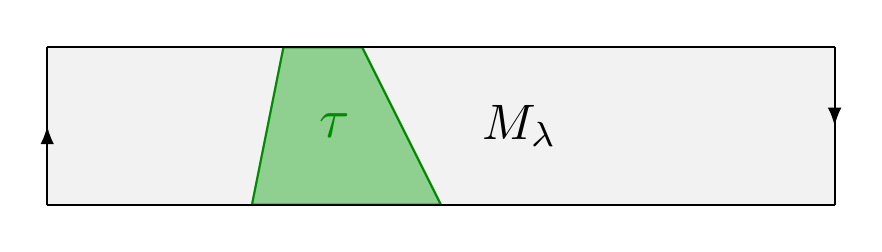
\begin{tikzpicture}[
    identified_edge/.style={
        decoration={
            markings,
            mark=at position 0.5 with {\arrow{Latex}}
        },
        postaction={decorate}
    },
    edge_label/.style={midway, auto, font=\small}
]

\def\squaresize{2}
\fill[gray!10] (0,0) -- (0,\squaresize) -- (5 * \squaresize, \squaresize) -- (5 * \squaresize,0) -- cycle;
\draw (0,0) rectangle (5 * \squaresize,\squaresize);

\fill[green!25!lightgray] (1.3 * \squaresize,0) -- (2.5*\squaresize,0) -- (2*\squaresize,\squaresize) -- (1.5*\squaresize,\squaresize) -- cycle;

\draw[green!55!black, thick] (1.3 * \squaresize,0) -- (2.5*\squaresize,0) -- (2*\squaresize,\squaresize) -- (1.5*\squaresize,\squaresize) -- cycle;
\draw[black, thick] (0,\squaresize) -- node[edge_label, above] {} (5 * \squaresize,\squaresize);
\draw[black, thick] (0,0)       -- node[edge_label, below]  {} (5 * \squaresize,0);
\draw[identified_edge, thick] (0,0)       -- node[edge_label, left]  {} (0,\squaresize);
\draw[identified_edge, thick] (5 * \squaresize,\squaresize) -- node[edge_label, right] {} (5 * \squaresize,0);
\node[green!55!black, scale=2] at (1.825*\squaresize,0.5*\squaresize) {$\tau$};
\node[black, scale=1.8] at (3 * \squaresize,0.5*\squaresize) {$M_\lambda$};



\end{tikzpicture}

\end{document}